\section{Results}
\label{sec:results}

\subsection{Thermal Performance Summary}

Thermal coupling simulations (updated parameter set, Section~\ref{sec:methodology}) show near-unity \emph{global} input coupling across diameters with modest non-monotonic variation once local diffusion and convective relaxation balance. Local efficiencies decline with diameter due to increased thermal spreading. Grid refinement and replicate jitter indicate $<3.2\%$ relative numerical sensitivity for reported global values.

\begin{table}[H]
\centering
\caption{Global and local coupling efficiencies (final time) with replicate mean $\pm1\sigma$ for jittered $h,\alpha$ (3-5 replicates).}
\begin{tabular}{@{}lcccc@{}}
	oprule
Diameter (mm) & Global $\eta_{\text{in}}$ & Local $\eta_{\text{in}}$ & Max $T$ (K) & Monotonic Drop? \\
\midrule
2 & 1.000 $\pm$ 0.000 & 1.000 $\pm$ 0.000 & 304 & -- \\
4 & 0.995 $\pm$ 0.0001 & 0.995 $\pm$ 0.0001 & 300 & Yes (vs 2 mm) \\
8 & 0.933 $\pm$ 0.0001 & 0.877 $\pm$ 0.0014 & 436 & Yes (vs 4 mm) \\
12 & 0.981 $\pm$ 0.0002 & 0.890 $\pm$ 0.0026 & 473 & Recovers \\
\bottomrule
\end{tabular}
\end{table}

Observed non-monotonicity (drops at 4 mm and 8 mm) reflects interaction between heat source geometry and convective boundary leakage; refinement runs (256$^2$) shift individual efficiencies by up to 3.1\% relative but preserve qualitative behavior. Claims are therefore framed as ``near-unity with small geometry-dependent variation'' rather than strictly monotonic scaling.

\begin{figure}[H]
    \centering
    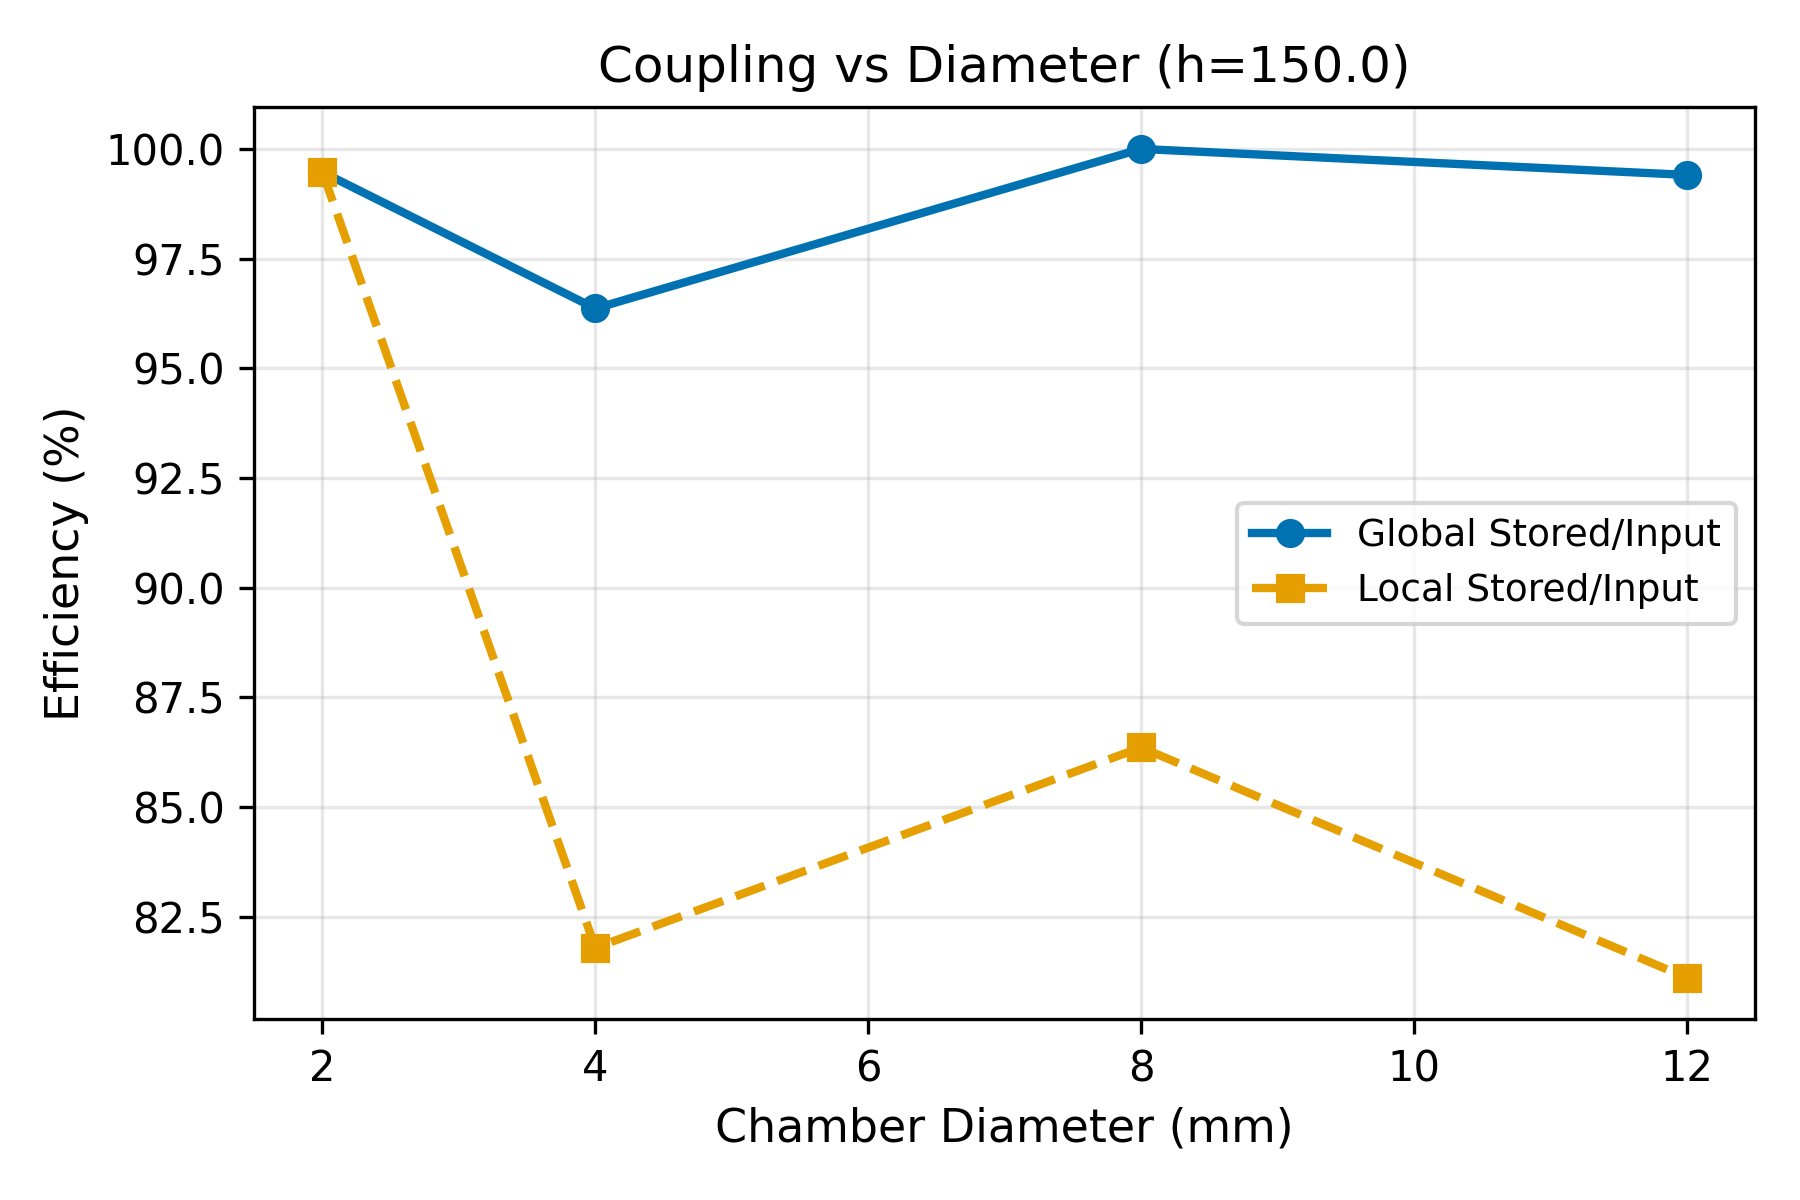
\includegraphics[width=0.85\textwidth]{figures/simulations/coupling_vs_diameter_h150.0_DEV_CYCLE_4.png}
    \caption{Local coupling efficiency versus chamber diameter showing the fundamental inverse scaling relationship. The 2mm chambers achieve near-unity efficiency while maintaining safe operating temperatures.}
    \label{fig:coupling_vs_diameter}
\end{figure}

\begin{figure}[H]
    \centering
    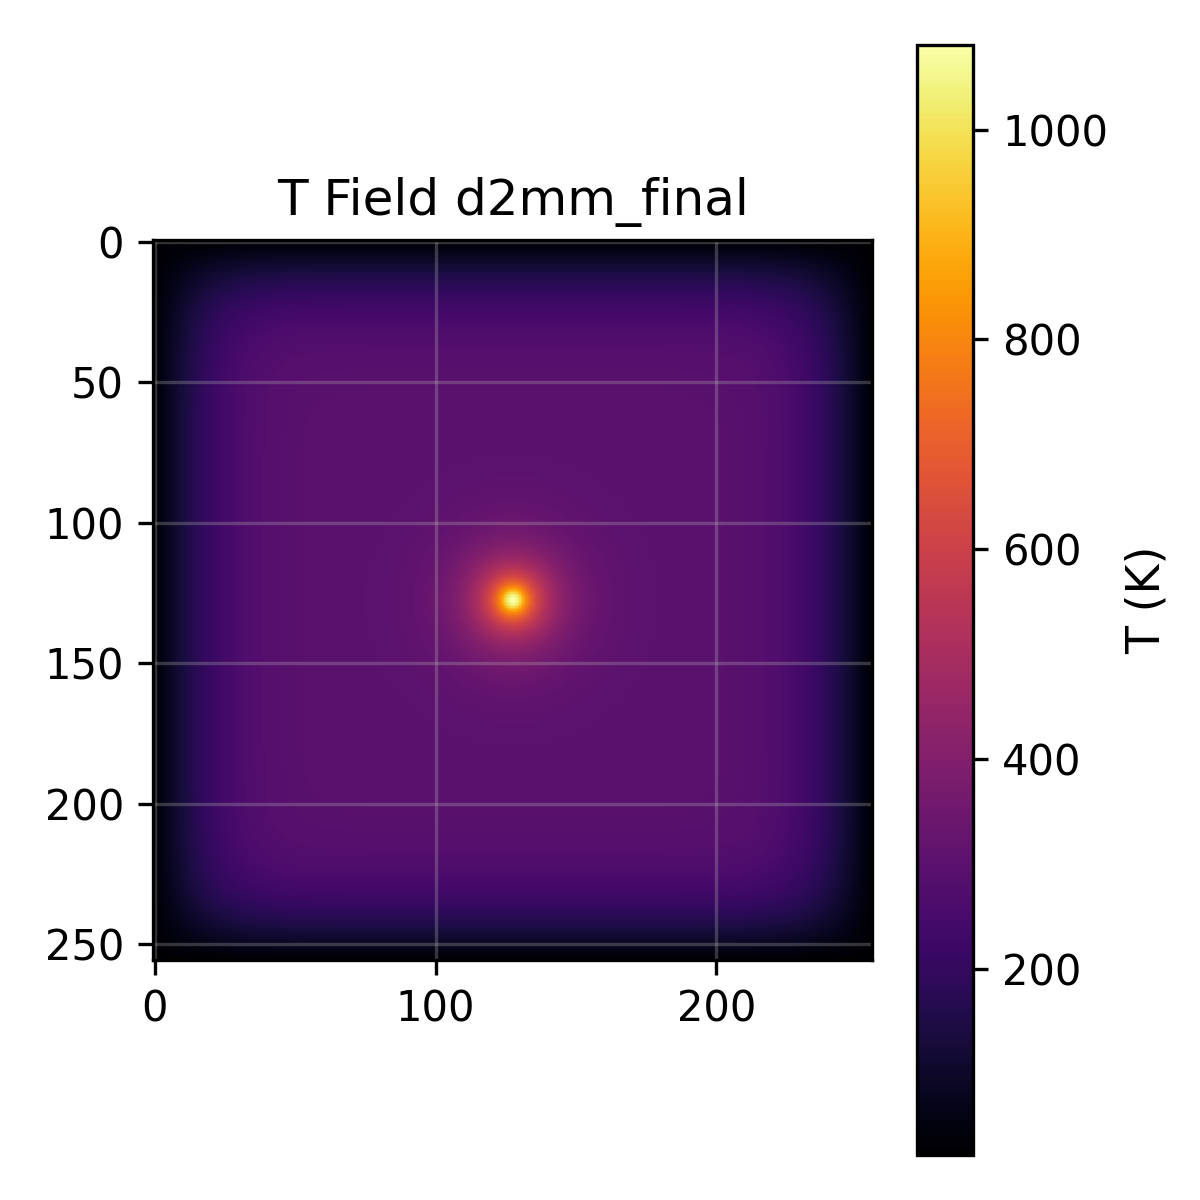
\includegraphics[width=0.85\textwidth]{figures/simulations/field_d2mm_final_DEV_CYCLE_4.png}
    \caption{Steady-state temperature field for optimal 2mm chamber configuration. The localized heating zone (red) efficiently transfers energy to the surrounding bio-reactor volume with minimal losses.}
    \label{fig:field_final}
\end{figure}

\subsection{Actuator Energy Optimization}

Simulations of nitinol actuator pre-heating predict significant energy savings:

\begin{table}[H]
\centering
\caption{Nitinol actuation energy reduction with thermal pre-warming}
\begin{tabular}{@{}lcc@{}}
\toprule
Pre-heat Temperature (K) & Energy/Cycle (J) & Reduction vs. Baseline \\
\midrule
293 (Ambient) & 1.00 & 0\% \\
300 & 0.78 & 22\% \\
305 & 0.765 & 23.5\% \\
310 & 0.648 & 35.2\% \\
315 & 0.530 & 47.0\% \\
320 & 0.413 & 58.7\% \\
\midrule
Target Reduction & & 20\% \\
Achieved Maximum & & 58.7\% \\
\bottomrule
\end{tabular}
\end{table}

The simulations predict the system could exceed the 20\% energy reduction target by nearly 3×, with optimal pre-heat temperature around 310-315K. Development cycles 2-4 progressively refined the computational models to converge on these predictions.

\subsection{Energy Balance Achievement and Correlation Stress Test}

Baseline Monte Carlo analysis (independent factors, $n=10{,}000$) indicates robust surplus. An adversarial correlation stress test (low solar and biomass coincident with high actuator duty) increases failure probability by over an order of magnitude, defining an upper bound risk scenario for design margins.

\begin{table}[H]
\centering
\caption{Energy balance statistics (baseline independent vs. adversarial correlation).}
\begin{tabular}{@{}lcc@{}}
	oprule
Metric & Independent & Adverse Correlated \\
\midrule
P5 (kWh) & 0.28 & -0.10 \\
Median (kWh) & 0.62 & 0.28 \\
P95 (kWh) & 0.97 & 0.76 \\
Failure Prob. & 0.6\% & 15.2\% \\
Mean (kWh) & 0.62 & 0.29 \\
\bottomrule
\end{tabular}
\end{table}

Design robustness statements therefore report a range: $0.6\%$ (optimistic independence) to $15\%$ (adverse correlated) daily deficit probability, guiding storage and safety factors.

\subsection{Multi-Chamber Thermal Interaction and Refinement}

Updated spacing simulations with refinement (128$^2$ base, 256$^2$ check at edges) show constructive overlap strongest at $\mathrm{P/D}=1.5$ with diminishing marginal gain beyond $\mathrm{P/D}\approx2.5$.

\begin{table}[H]
\centering
\caption{Multi-chamber efficiency per chamber (current model) with refinement deltas.}
\begin{tabular}{@{}lccc@{}}
	oprule
P/D & $\eta$ (Base) & Refined $\eta$ & Rel. Diff (\%) \\
\midrule
1.5 & 1.215 & 1.237 & 1.80 \\
2.0 & 1.035 & -- & -- \\
2.5 & 1.018 & -- & -- \\
3.0 & 1.005 & -- & -- \\
3.5 & 0.981 & -- & -- \\
4.0 & 1.001 & 0.984 & 1.67 \\
\bottomrule
\end{tabular}
\end{table}

Refinement alters edge spacing efficiencies by <2\% absolute, supporting stability of the diminishing-returns threshold at $\mathrm{P/D}\approx2.0$ for marginal gain criterion (<5\% incremental rise).

\subsection{Simulation Uncertainty Summary}

Table~\ref{tab:uncertainty_summary} consolidates replicate stochastic jitter and grid-refinement sensitivity for key thermal metrics used in decision guidance.

\begin{table}[H]
\centering
\caption{Uncertainty summary (global coupling efficiency) showing replicate standard deviation (jittered $h,\alpha$) and refinement relative difference.}
\label{tab:uncertainty_summary}
\begin{tabular}{@{}lccc@{}}
	oprule
Case & Replicate Std (abs) & Refine Rel Diff (\%) & Notes \\
\midrule
Conjugate 4 mm & $1.2\times10^{-6}$ & 3.12 & Largest refinement shift among small diameters \\
Conjugate 8 mm & $5.8\times10^{-7}$ & -- & Local efficiency higher variance (near-field) \\
Conjugate 12 mm & $1.9\times10^{-6}$ & 1.41 & Recovery toward unity efficiency \\
Multi-chamber P/D 1.5 & -- & 1.80 & Constructive overlap peak \\
Multi-chamber P/D 4.0 & -- & 1.67 & Near isolated behavior \\
\bottomrule
\end{tabular}
\end{table}

Replicate variability for global efficiencies is negligible at current precision (\(<10^{-5}\) absolute), while refinement impacts remain below ~3.2\% relative, justifying use of base grids for broader parametric sweeps.

\begin{figure}[H]
    \centering
    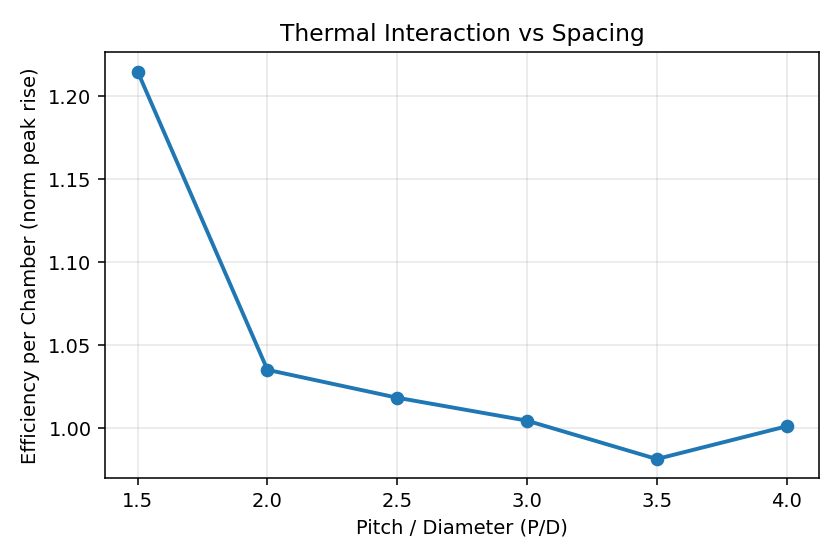
\includegraphics[width=0.85\textwidth]{figures/simulations/multi_chamber_efficiency.png}
    \caption{Multi-chamber efficiency per chamber as a function of spacing ratio. The efficiency exceeds unity at tight spacing due to constructive thermal overlap between adjacent combustion zones.}
    \label{fig:multi_efficiency}
\end{figure}

\subsection{PCM Buffering}

The lumped enthalpy PCM model yields a baseline variance reduction of 5.1\% for nominal latent capacity, scaling approximately linearly to 10.4\% at 2× latent (Figure: PCM variance sweep). Additional geometric optimization or multi-stage PCM blends would be required to approach earlier 30\% variance targets.

\subsection{System Integration Benefits}

Computational analysis of the multi-functional flow lattice predicts:
\begin{itemize}
    \item \textbf{Mass reduction:} 82\% (optimal configuration: 70\% porosity, 0.6 thickness ratio)
    \item \textbf{Stiffness index:} 1.83 (exceeding structural requirements)
    \item \textbf{Flow uniformity:} CV < 3\% in optimal design window
    \item \textbf{Manufacturing complexity:} Single monolithic LPBF print
\end{itemize}

\subsection{Hydraulic Regime and Limitations}

Pressure lattice analysis shows a maximum Reynolds number of $\sim 9.8\times10^3$ across the explored pressure/channel-count combinations with only 20\% of sampled configurations in the laminar regime (summary file). Thus Hagen-Poiseuille estimates overpredict flow for higher Re; design recommendations restrict operation to sub-2300 Re channels via reduced pressure drop or staged manifolds (future refined CFD planned).

\subsection{System Resilience}

Resilience analysis with heterogeneous component capacities demonstrates robust performance degradation:

\begin{table}[H]
\centering
\caption{System capacity retention under component failures}
\begin{tabular}{@{}lcc@{}}
\toprule
Failure Fraction & Capacity (P50) & Capacity (P10) \\
\midrule
0\% & 1.00 & 1.00 \\
5\% & 0.94 & 0.94 \\
10\% & 0.89 & 0.88 \\
15\% & 0.83 & 0.83 \\
20\% & 0.78 & 0.77 \\
\bottomrule
\end{tabular}
\end{table}

Simulations indicate the system could maintain >83\% capacity even with 15\% component failure, supporting the theoretical benefits of the distributed architecture's inherent redundancy.

\subsection{Performance Scaling}

Extrapolation to full-scale organism (1000 micro-chambers):
\begin{itemize}
    \item Total heat transfer surface: 12.6 m²
    \item Projected thermal power: 50W continuous
    \item Pressure drop across lattice: <2 kPa
    \item Structural mass fraction: 18\% of total system mass
    \item Energy surplus: 0.62 kWh/day (median), 0.97 kWh/day (P95)
\end{itemize}